\chapter{Point cloud algorithms}\label{chap:point-cloud-algorithms}



\section*{}

This chapter presents the main algorithms that can be used to retrieve and analyze point clouds in the context of a robot localization system.

It starts by giving an overview of how point clouds can be acquired and efficiently searched. Then moves on to the preprocessing methods that can be applied to improve the quality of the sensor data. Later on, two approaches capable of performing point cloud registration are presented. The first uses geometric features to compute the initial point cloud alignment, and the second employs error minimization techniques to calculate the final registration. Lastly it is discussed how to segment outliers and how to dynamically updated the reference point cloud using new sensor data.



\section{Point cloud acquisition}

Point clouds can be retrieved with a wide range of sensors with varying levels of precision and assembly time. They usually rely on time of flight or trilateration / triangulation techniques to compute distances to environment objects, which in combination with the sensor position and orientation allows to retrieve the Euclidean coordinates of the scene points. Some sensors can also capture the point's reflectance or color, which can be very useful in segmentation techniques and point cloud feature algorithms.


\subsection{\glsentrydesc{tof} systems}

Time of flight systems measure the time that a wave takes to leave the sensor, hit the environment and return to the sensor. Knowing the speed at which the wave travels, the distance between the two can be easily computed.

Several time of flight systems were developed over the years that use different types of waves according to the environment in which they were designed to operate. Some use high precision light waves (\gls{lidar}) while others employ less accurate radio / sound waves (\gls{radar} / \gls{sonar}). \cref{sec:localization-methods_tof-methods} gives a more detailed description of these systems.


\subsection{Triangulation and trilateration systems}

Triangulation systems measure angles to a given point from several origins in order to compute the Euclidean coordinates of an environment object. Trilateration is similar but uses distances instead of angles. These methods are useful when the sensor orientation is not known or when there are two different views of the environment (stereo cameras and structured light scanners). \Cref{sec:localization-methods_trilateration-methods} introduces some of these systems.



\section{Point cloud search data structures}

Most of the point cloud algorithms use neighbor searches to analyze the surroundings of a given point. As such, efficient data structures are needed to speedup these operations, in order to execute the algorithms efficiently.


\subsection{Voxel grids}

A voxel grid is a three dimensional space partition data structure that splits the Euclidean space into regular voxels (volume pixel). It can be built very fast but is not very efficient for sparse point clouds. \Cref{fig:point-cloud-algorithms_voxel-grid} shows how the voxel size affects the level of detail of point clouds.

\begin{figure}[H]
	\centering
	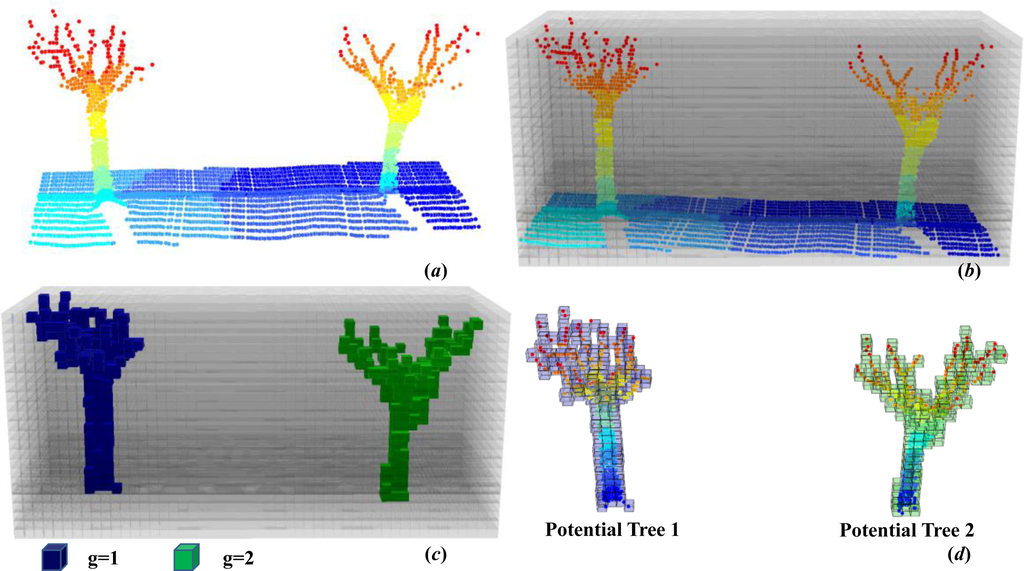
\includegraphics[width=\textwidth]{point_cloud_algorithms/voxel_grid}
	\caption{Voxel grid applied over trees point clouds \cite{Wu2013}}
	\label{fig:point-cloud-algorithms_voxel-grid}
\end{figure}



\subsection{Octrees}

An octrees is a hierarchical space partition technique that adapts its tree data structure to the distribution of points in the cloud. It accomplishes this by recursively dividing each voxel in 8 octants until the tree depth is reached or when there is no more points in that region of space. This can be seen in \cref{fig:point-cloud-algorithms_octree} in which areas with no points have large voxels while areas with high point density have much smaller voxels.

%\afterpage{
\begin{figure}[H]
	\centering
	\begin{minipage}[h]{.495\textwidth}
		\centering
		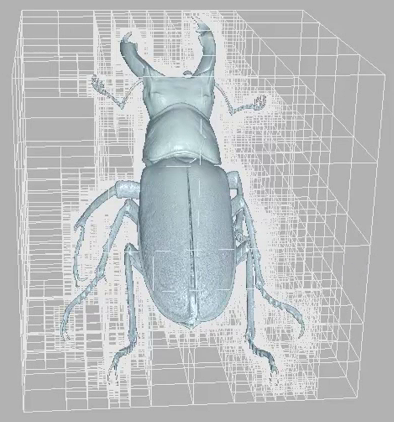
\includegraphics[width=0.55\textwidth]{point_cloud_algorithms/octree_1}
	\end{minipage}\hfill
	\begin{minipage}[h]{.495\textwidth}
		\centering
		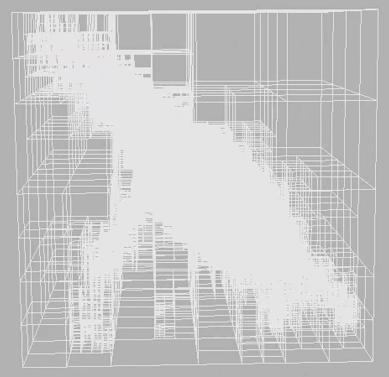
\includegraphics[width=0.6\textwidth]{point_cloud_algorithms/octree_2}
	\end{minipage}
	\caption{Octree of a stag beetle\protect\footnotemark}
	\label{fig:point-cloud-algorithms_octree}
\end{figure}
\footnotetext{\url{http://blog.mpanknin.de/?p=753}}
%}



\subsection{k-d trees}

A k dimensional tree is a space partition technique that can organize points with k dimensions. It is a generic data structure that can be used for 2D and 3D points (examples in \cref{fig:point-cloud-algorithms_2d-tree} and \cref{fig:point-cloud-algorithms_3d-tree}) as well as any other type of data that have an arbitrary number of dimensions (such as point cloud feature descriptors).

The binary k-d tree is built by successively selecting the median point in each axis until all points are inserted in the tree (the selection of the next axis is performed in a circular way, which in the case of three dimensional data means that after processing the z axis, the x axis would be selected).

%\afterpage{
\begin{savenotes}
\begin{figure}[ht]
	\centering
	\begin{minipage}[h]{0.495\textwidth}
		\centering
		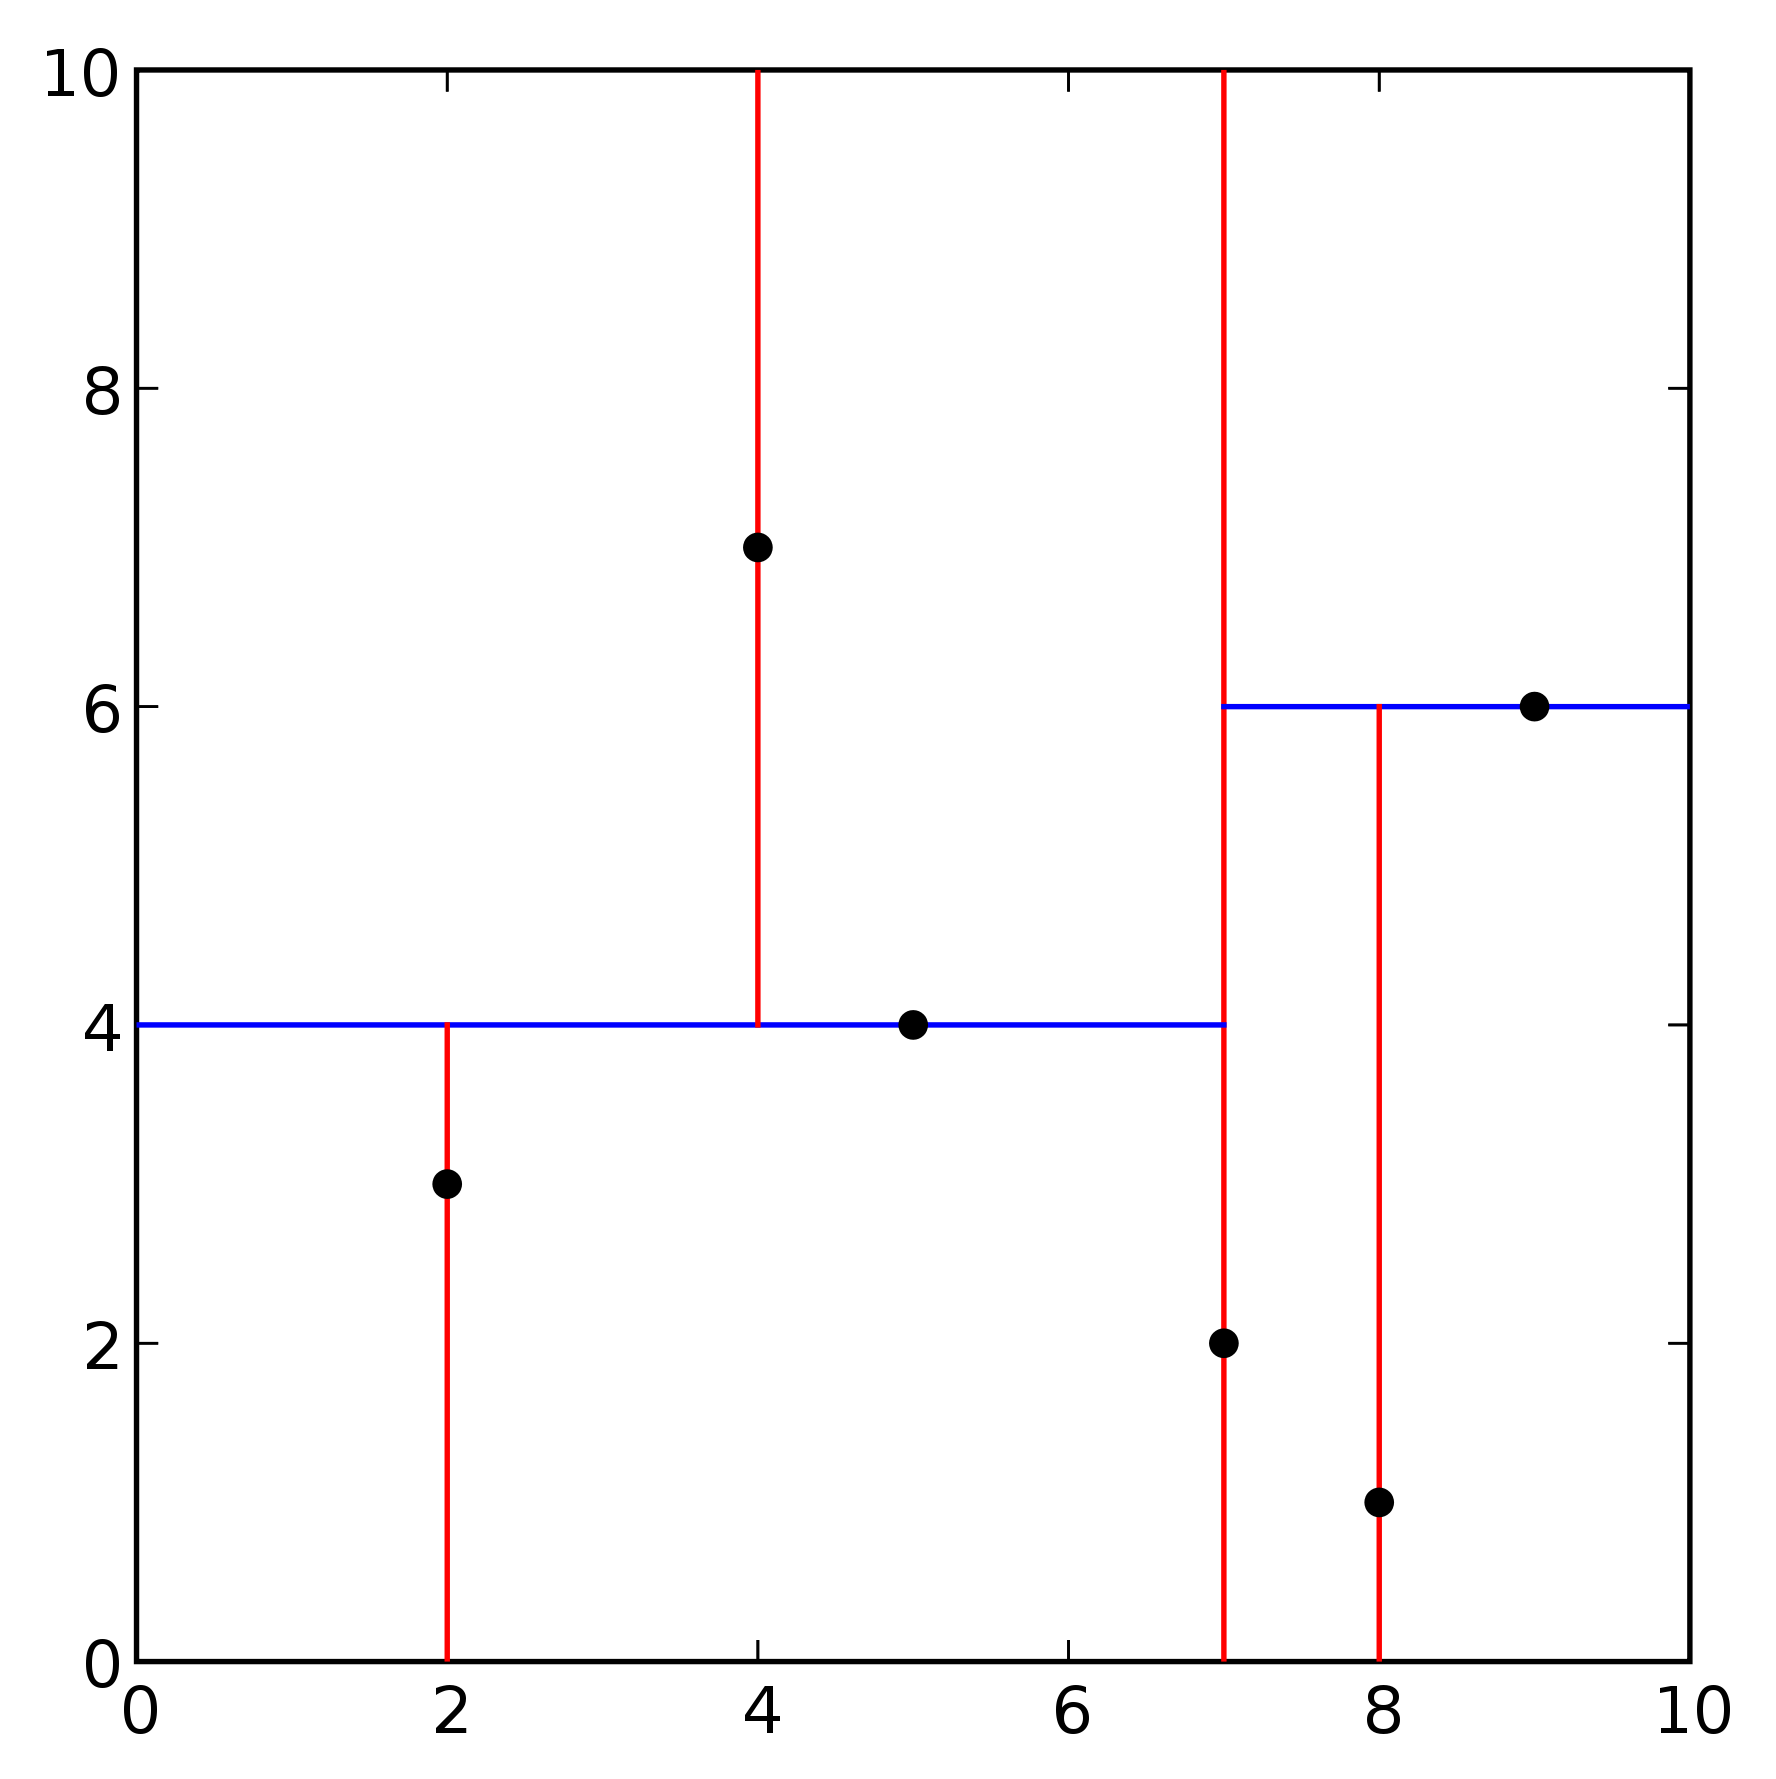
\includegraphics[width=0.6\textwidth]{point_cloud_algorithms/kdtree_2d}
		\caption{2-d tree\protect\footnotemark}
		\label{fig:point-cloud-algorithms_2d-tree}
	\end{minipage}\hfill
	\footnotetext{\url{http://en.wikipedia.org/wiki/K-d_tree}}
	\begin{minipage}[h]{0.495\textwidth}
		\centering
		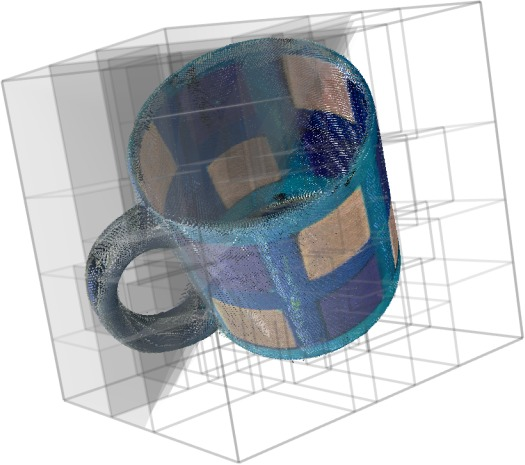
\includegraphics[width=0.65\textwidth]{point_cloud_algorithms/kdtree_3d}
		\caption{3-d tree\protect\footnotemark}
		\label{fig:point-cloud-algorithms_3d-tree}
	\end{minipage}
	\footnotetext{\url{http://docs.pointclouds.org/trunk/group__kdtree.html}}
\end{figure}
\end{savenotes}
%}



\section{Point cloud preprocessing}

Point cloud data that comes from laser sensors can have a considerable amount of noise and an unnecessary level of detail. To cope with these problems, several preprocessing algorithms can be applied, ranging from simple point cloud downsampling to the more advanced outlier removal and surface reconstruction methods.


\subsection{Point cloud downsampling}

Downsampling methods aim to reduce the number of points while maintaining the surface structure of a given point cloud. They can be used to adjust the level of detail according to the point cloud registration precision required.


\subsubsection{Voxel grid sampling}

A voxel grid is a uniform space partition technique that can be used to cluster points according to their Euclidean coordinates. As can be seen in \cref{fig:point-cloud-algorithms_voxel-grid-downsampling}, it is a very effective method to control the level of detail of a point cloud because it gives the ability to specify the maximum number of points that a region in space should have.

The point cloud downsampling is achieved by replacing each cluster with a single point. The selection of this point can be very fast if the voxel center is used, but computing the centroid of the cluster yields better results because it represents the underlying surface with more accuracy and it attenuates errors in the sensors measurements.


%\afterpage{
\begin{figure}[H]
	\centering
	\begin{minipage}[h]{0.495\textwidth}
		\centering
			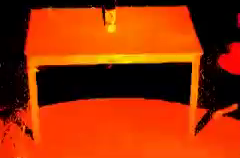
\includegraphics[width=0.78\textwidth]{point_cloud_algorithms/voxel_grid_downsampling_1}
	\end{minipage}\hfill
	\begin{minipage}[h]{.495\textwidth}
		\centering
	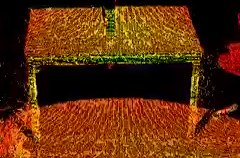
\includegraphics[width=0.78\textwidth]{point_cloud_algorithms/voxel_grid_downsampling_2}
	\end{minipage}
	\caption{Table point cloud before (left) and after (right) voxel grid downsampling\protect\footnotemark}
	\label{fig:point-cloud-algorithms_voxel-grid-downsampling}
\end{figure}
\footnotetext{\url{http://pointclouds.org/documentation/tutorials/voxel_grid.php}}
%}



\subsubsection{Random sampling}

Random sampling \cite{Vitter1984} is a fast downsampling method that randomly selects points from the input cloud until the specified number of samples is reached. This has the advantage of using real measures instead of downsampled approximations, but also means it is more sensible to sensor measurements noise. However, for outdoor environments or very complex scenes, using the real measurements can be preferable than using cluster centroids because the voxels may not have the necessary resolution or may have a prohibitive computational cost.


\subsubsection{Covariance sampling}

Covariance sampling \cite{Gelfand} is a subsampling method that aims to create a stable downsampled point cloud to be registered with \gls{icp} algorithms. It incrementally builds the downsampled point cloud while trying to keep the 6 eigenvalues of the covariance matrix as close to each other as possible.

The resultant point cloud has the desired number of points and is stable enough to be matched with \gls{icp} point to plane algorithms.


\subsection{Outlier removal}

Laser range finders can perform measurements with millimeter accuracy, but they have some limitations that can lead to the creation of outliers \cite{Sotoodeh2006}.

One of those limitations can produce shadow points around objects boundaries. This is due to the fact that a portion of the laser beam may hit the object boundary and other part may hit other areas in the object background. And given that most laser range finders use a weighted sum of several beams, this can yield measurements that are not associated with any real object (outliers). \Cref{fig:point-cloud-algorithms_voxel-grid-downsampling} shows a considerable amount of these shadow points close to the front table legs. Another issue is related to the angle in which the laser beam hits the objects. If the incidence angle is very low, then it may be difficult to detect if the beam had ambient reflections. This can significant increase the measurements noise or even lead to the creation of outliers. Other less common problem is associated with the material properties of the surfaces. For example, objects with very high or very low reflectance, such as metals or glass, can increase the measurements noise. Moreover depending on the combination of surface geometry, material and incidence angle, some objects may even be undetectable by laser range finders.

Given the negative effect that outliers have in object segmentation and registration algorithms, they should be removed in a preprocessing stage. There are several approaches to perform outlier detection and removal \cite{YangZhang2010}, ranging from simple distance thresholds to more robust statistical analysis. The next sections present some of then that can be useful in a localization system.


\subsubsection{Distance filter}

Given that laser range finders have a maximum distance for their measurements, it is wise to remove points that are close or beyond this limit. Moreover, it may be useful to remove points that are too close to the sensor, because they may belong to the robot itself and not the environment.

This can be achieved by applying a minimum and maximum threshold to the distances returned by the laser sensor (before converting then to Euclidean points).


\subsubsection{Passthrough filter}

A passthrough filter can select or remove points according to their properties.

For outlier removal, it can be used to select points that are within a given bounding box (useful when we already know what area of the environment we want to analyze) or remove points that don't have the appropriate intensity or color.


\subsubsection{Radius outlier removal filter}

The radius outlier removal filter deletes points that don't have a minimum number of neighbors within a specified radius distance. It can be useful when the point density is known and is very effective in removing isolated points.


\subsubsection{Statistical outlier removal filter}

The statistical outlier removal filter \cite{Rusu2010a} performs a global analysis of the distances between points and discards the ones that don't follow the global distance distribution.

It is a robust filter that adapts itself to the point cloud density and is very effective in removing shadow points. To do so, it computes the mean distance that each point has to a given number of neighbors and builds a global distance distribution (example in \cref{fig:point-cloud-algorithms_statistical-outlier-removal}). Then, assuming that the distribution is Gaussian, it discards the points that have a distance higher than a given threshold (that is a percentage of the standard deviation of the distance distribution).

%\afterpage{
\begin{figure}[H]
	\centering
	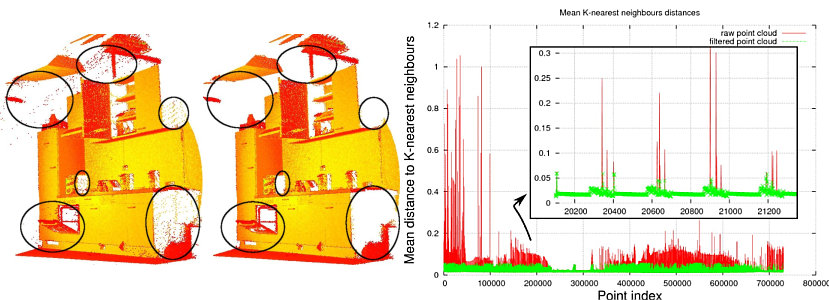
\includegraphics[width=\textwidth]{point_cloud_algorithms/statistical_outlier_removal}
	\caption{Statistical outlier removal filter\protect\footnotemark}
	\label{fig:point-cloud-algorithms_statistical-outlier-removal}
\end{figure}
\footnotetext{\url{http://pointclouds.org/documentation/tutorials/statistical_outlier.php}}
%}


\subsection{Surface and object reconstruction and resampling}

Depending on the level of sensor noise and amount of outliers present in a given point cloud, it may be necessary to employ surface reconstruction techniques to fill gaps in sensor data or correct measurements errors. The next sections introduce some of the most common techniques to achieve these goals.


\subsubsection{Object recognition and model fitting}

One of the most advanced techniques that can be used to fill gaps in sensor data relies on object recognition or model fitting. These techniques are usually applied to small objects that have only the front side visible. They are useful when it is necessary to know the approximate shape of objects. However, they require a priori knowledge about the types of shapes or objects that are present in the scene.


\subsubsection{Moving Least Squares}\label{sec:point-cloud-algorithms_mls}

Moving least squares \cite{Alexa2003} is a surface reconstruction algorithm that uses higher order bivariate polynomials to fit surfaces to a given set of points. It can be used to fill possible gaps in sensor data, smooth the point cloud (shown in \cref{fig:point-cloud-algorithms_mls-smoothing}), refine surface normals (shown in \cref{fig:point-cloud-algorithms_mls-nomal-refinement}) and perform downsampling or upsampling.

Surface reconstruction can also be useful when the point cloud is built from several laser scans with different origins and registered with some alignment errors. In \cref{fig:point-cloud-algorithms_mls-nomal-refinement} can be seen that the normal estimation is not very accurate in the regions of overlap between different scans. This can be solved by estimating the normals using the surfaces computed by the moving least squares algorithm instead of using the point's neighbors.


%\afterpage{
\begin{figure}[H]
	\centering
	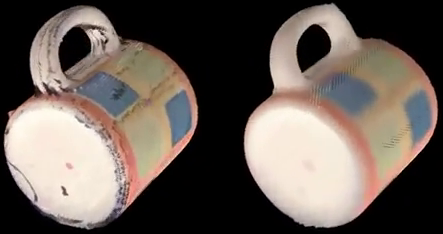
\includegraphics[width=0.57\textwidth]{point_cloud_algorithms/mls_smoothing}
	\caption{Surface smoothing using moving least squares algorithm\protect\footnotemark}
	\label{fig:point-cloud-algorithms_mls-smoothing}
\end{figure}
\footnotetext{\url{http://pointclouds.org/documentation/tutorials/resampling.php}}
%}

%\afterpage{
\begin{figure}[H]
	\centering
	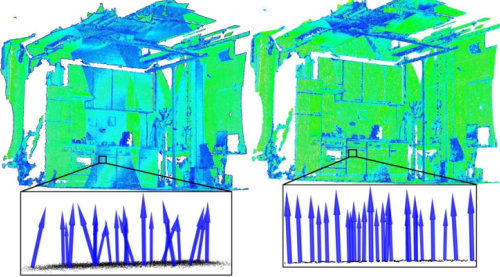
\includegraphics[width=0.57\textwidth]{point_cloud_algorithms/mls_nomal_refinement}
	\caption{Surface normals refinement using moving least squares algorithm \cite{Rusu2010a}}
	\label{fig:point-cloud-algorithms_mls-nomal-refinement}
\end{figure}
%}



\section{Point cloud features}

Aligning two point clouds with overlapping views of the environment requires the establishment of point correspondences. If both point clouds have similar sensor origins, these can be determined with nearest neighbor's searches and filtered with correspondence rejectors (using other point properties such as reflectance and color). But if they were acquired in two very different positions, then more advanced techniques must be employed.

One of those techniques uses histograms to describe the geometric properties of the environment around a given point. This allows points to be matched even if they have completely different Euclidean coordinates. Also, by using histograms and sampling techniques, these descriptors are much more robust against sensor noise and varying level of point density. However, these advantages come with a heavy computational cost, and as such, point descriptors should only be computed on the most descriptive areas of the environment.

Identifying these environment points is known as feature / keypoint detection, and usually involves finding interesting points, such as corners and edges. Besides uniqueness, these points must also be repeatable. This means that the detection algorithms should be able to find the same points even if they are present in different point clouds with sensor noise and varying point density. This is of the utmost importance, because if the same keypoints are not identified on both clouds, then matching the point descriptors will likely fail.

The next sections introduce some of the most used algorithms for normal estimation, keypoint detection and point description.


\subsection{Surface normal estimation}

Surface normals provide information about the orientation of their underlying geometry and are widely used as the basis for other point descriptors. They can be computed using plane fitting methods or using more advanced techniques such as the one presented in \cref{sec:point-cloud-algorithms_mls}.

These algorithms analyze the neighborhood of a given point in order to compute the surface normal, and as such, the correct specification of what points should be included in the estimation is crucial to achieve accurate results. This depends on the environment geometry and the level of detail that is required, and is usually done by specifying a radius distance (example in \cref{fig:point-cloud-algorithms_surface-normals}) or by limiting the number of neighbor points to use.

\begin{figure}[H]
	\centering
	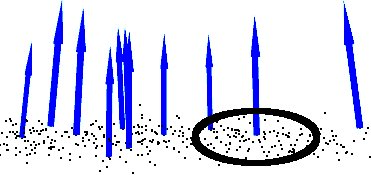
\includegraphics[width=0.5\textwidth]{point_cloud_algorithms/surface_normals}
	\caption{Point neighborhood for normal estimation \cite{Rusu2010a}}
	\label{fig:point-cloud-algorithms_surface-normals}
\end{figure}

